A continuació s'expliquen diverses implementacions interessants, o bugs curiosos i la seva subseqüent solució.
\section{Observer}
La implementació del observador és una de les parts que es va fer més tard, i és una implementació on es demostra part de la potència de C++, i en concret, C++20 / Modern C++.
\\
\begin{lstlisting}[language=C++]
using eventArgs = std::variant<
	std::tuple<entt::entity, entt::entity, double>,
	std::tuple<universeNode*, entt::entity, double>,
	std::tuple<universeNode*, universeNode*, double>,
	entt::entity
>;
\end{lstlisting}
Primer de tot aquí creem un tipus de dades anomenat eventArgs, el qual representarà els arguments que un esdeveniment pot enviar als subscriptors.
Std::variant a vegades anomenat "sum type" podriem descriure'l com l'equivalent a un \textit{union} amb \textit{type safety}. 
Així doncs, una variable del tipus eventArgs podrà contenir una std::tuple d'algun dels tipus especificats, o un entt::entity.
\\
\begin{lstlisting}[language=C++]
enum class eventType{
	COLLISION_EE,
	COLLISION_NE,
	COLLISION_NN,
	PROJECTILEHIT,
	PROJECTILEBOUNCE,
	_SIZE,
};
\end{lstlisting}
Tot seguit definim el enum class eventType, que especificara els diversos tipus d'esdeveniments que el nostre observador pot gestionar.
\\
\begin{lstlisting}[language=C++]
namespace {
	consteval std::array<size_t,(unsigned)eventType::_SIZE> 
    _observertypetable(std::array<std::pair<eventType,eventArgs>,
    (unsigned)eventType::_SIZE> args){
		  std::array<size_t,(unsigned)eventType::_SIZE> result;
  		for(auto& val : args){
	  		result[(unsigned)val.first] = val.second.index();
  		}
	  	return result;
	  }
}
\end{lstlisting}
A continuació tenim una funció \textit{consteval} dins un espai de noms anònim, que evita que la funció sigui accessible fora d'aquest arxiu.
L'especificador \textit{consteval} avisa al compilador que la funció no té efectes secundaris, i pot ser avaluada en temps de compilació en cas de ser necessari.
La funció en sí retorna un array amb tamany igual al nombre de tipus d'esdeveniments diferents que tenim a eventType, i a cada posició conté una variable size\_t. 
Pren per argument un array que conté parelles de eventType i eventArgs, els quals relacionarà per retornar l'array resultant.
\\
Per crear aquest resultat primer de tot l'inicialitza.
Després itera per cada parella de eventType i eventArgs.
Al array resultant coloca a la posició indexada pel valor del eventType un valor de tipus size\_t, aquest valor l'obté de cridar index() al variant, que serveix com a una pseudo-reflexió i retorna l'índex del tipus dins del variant.
Un cop ha iterat per totes les parelles retorna l'array que ha construït.
\\

\begin{lstlisting}[language=C++]
constexpr std::array<size_t,(unsigned)eventType::_SIZE> _eventLUT = _observertypetable(
  std::array<std::pair<eventType,eventArgs>,(unsigned)eventType::_SIZE>{
	std::make_pair(eventType::COLLISION_EE,std::tuple<entt::entity,entt::entity, double>()),
	std::make_pair(eventType::COLLISION_NE,std::tuple<universeNode*,entt::entity, double>()),
	std::make_pair(eventType::COLLISION_NN,std::tuple<universeNode*,universeNode*, double>()),
	std::make_pair(eventType::PROJECTILEHIT,std::tuple<entt::entity,entt::entity, double>()),
	std::make_pair(eventType::PROJECTILEBOUNCE,entt::entity())
});
\end{lstlisting}
Tot seguit creem una LUT que consisteix en l'array obtingut al cridar la anterior funció. La funció la cridem amb un std::array que creem \textit{in-place} que conté parelles de eventType i eventArgs.
\\
\begin{lstlisting}[language=C++]
class observer {
public:
  static void registerSubscriber(eventType t, std::function<void(eventArgs args)> f,void* owner){
    if(!_subscribers[(unsigned)t].contains(owner))
		  _subscribers[(unsigned)t].emplace(owner,f);
  }
  static void deleteSubscriber(eventType t, void* owner){
    if(_subscribers[(unsigned)t].contains(owner))
      _subscribers[(unsigned)t].erase(owner);
  }


	template <eventType E,typename T>
	static void sendEvent(T args)
	{
		static_assert(eventArgs(T()).index()==_eventLUT[(unsigned)E]);
		for(auto& sub : _subscribers[(unsigned)E]){
			sub.second(eventArgs(args));
		}
	}

private:
	static std::array<std::unordered_map<void*,std::function<void(eventArgs args)>>,
  (unsigned)eventType::_SIZE> _subscribers;
};
\end{lstlisting}
Finalment tenim el observer en sí. Les funcions registerSubscriber i deleteSubscriber simplement afegeixen un subscriptor al observador o l'esborren.
Tenim un std::array que per cada tipus de esdeveniment conté un std::map que relaciona subscriptors amb funcions a cridar. El void* és un handle que l'objecte que s'ha subscrit ha donat al subscriure's, podria interpretar-se com un "reverse handle".
\\
La funció interessant és sendEvent. És una funció genèrica depenent del tipus T i el tipus d'esdeveniment E. Primer de tot es fa una asserció estàtica utilitzant la \textit{lookup table} que abans hem emplenat. Aquesta asserció comprova en temps de compilació que l'esdeveniment que s'envia s'adigui a les dades que s'envien junt amb ell.
En temps d'execució el que es farà serà iterar per tots els subscriptors d'aquell tipus d'esdeveniment, i es cridarà la funció associada a cada subscriptor.
\\
D'aquesta manera tenim una implementació d'un observador amb poc codi innecessari, senzilla i amb comprovació de tipus en temps de compilació.
\section{universeNode::getLocalPos}
La funció universeNode::getLocalPos serveix per obtenir la posició local a un node específic, donada una posició qualsevol i el seu node pare.
\begin{lstlisting}[language=C++]
fdd universeNode::getLocalPos(fdd f, universeNode* u) const
{
	assert(!std::isnan(_position.x));
	if (u == this)
		return f;
	else
	{
		fdd transform = f;
		const universeNode* transformLocal = this;

		while (transformLocal != u) { // while transformLocal isn't f's parent (u)
			if (u && u->_depth > transformLocal->_depth) {//should move u
				transform += u->_position;
				u = u->_parent;
			}
			else {// move transformLocal
				transform -= transformLocal->_position;
				transformLocal = transformLocal->_parent;
			}
		}
		return transform;
	}
}
\end{lstlisting}
Primer de tot creem una fdd anomenada transform, que representarà la transformació que anem acumulant al atravessar l'arbre de nodes, i també crearem una punter al pare actual de la transformació que estem construïnt.
Per tal d'evitar la pèrdua de precisió fent transformacions innecessaries, el que farem serà trobar el camí més curt atravessant l'arbre cap amunt des de orígen i destí. Un cop els dos pares coincideixin haurem arriat al objectiu.
Sempre mourem primer cap amunt la posició que estigui relativa a un node més profund, i en cas d'empat mourem l'origen. A l'hora de moure una de les posicions el que farem serà restar o sumar la posició del node actual a la transformació, depenent de si estem pujant l'origen o el destí. També actualitzarem la variable transformLocal o `u' cap al nou pare, depenent de quin haguem mogut.
Quan les transformLocal i `u' siguin el mateix node sabrem que hem aconseguit arribar al objectiu, i podrem retornar la transformació que hem anat construïnt com a resultat.

\section{terrainPainterGenerator::getChunk(const point3Di& p)}
\begin{lstlisting}[language=C++]
terrainChunk terrainPainterGenerator::getChunk(const point3Di& p)
{
	if (p.z < 0 || fdd{ 0,0,0,0 }.distance2D(fdd{ (double)(p.x) * config::chunkSize,
    (double)(p.y) * config::chunkSize,0,0 }) > (_diameter / 2)*config::chunkSize)
	{
		return terrainChunk();
	}

	terrainChunk chunk(p);

	for (int x = 0; x < config::chunkSize; ++x) {
		for (int y = 0; y < config::chunkSize; ++y) {
			if (fdd{ 0,0,0,0 }.distance2D(fdd{ (double)(p.x * config::chunkSize) + x,
        (double)(p.y * config::chunkSize) + y,0,0 }) <= _diameter / 2)
			{
				double noise = getNoise({ (p.x * config::chunkSize) + x,
          (p.y * config::chunkSize) + y });
				for (int z = 0; z < config::chunkSize; ++z) {
					unsigned int currentHeight = p.z * config::chunkSize + z;
					chunk.setBlock({&_terrainPainter.getBlock(currentHeight, noise),
            (blockRotation)(rand()%4)}, point3Di{ x,y,z });
				}
			}
		}
	}
	if(_liquidLevel>0)
		fillLiquid(chunk, p, _liquidLevel);
	chunk.setLoaded();
	chunk.clearDirtyFlag();
	return chunk;
}
\end{lstlisting}
Aquesta és la implementació de la funció que genera els chunks de terreny amb terrainPainterGenerator.
El seu funcionament és el següent:
\begin{enumerate}
  \item Es comprova que el chunk a generar sigui vàlid, i si es troba fora dels límits del terreny es retorna un chunk buit.
  \item En cas contrari, creem el chunk buit amb la posició que li correspon.
  \item Tot seguit iterem per les columnes de blocs en els eixos X i Y.
  \item Comprovem que el bloc a assignar estigui dins dels límits del generador, i en cas contrari ometem la generació d'aquesta columna de blocs.
  \item Obtenim el nivell de soroll a partir del generador de gradient de soroll en les coordenades X i Y actuals.
  \item Iterem pels blocs de la columna de blocs, i els assignem segons el bloc que el terrainPainter ens indiqui per aquella alçada i nivell de soroll.
  \item Un cop assignats els blocs, emplenem de líquid els blocs d'aire en cas que aquells blocs es trobin sota el nivell del mar.
  \item Finalment marquem el chunk com a carregat i net i el retornem.
\end{enumerate}
\section{Bugs}
Al llarg del desenvolupament del projecte s'han arreglat gran quantitat de \textit{bugs}, a continuació es detallen alguns dels més destacables.
\subsection{Pèrdua de precisió al calcular òrbites}
Degut a la gran escala del univers, el càlcul d'òrbites d'alguns cossos es feia de forma incorrecte a causa de falta de precisió en els nombres de coma flotant (IEEE 754-2008).
El problema originava de la falta de precisió al calcular el moviment en cossos llunyans al seu node pare, en els que l'increment de posició en 33ms era massa petit, i al afegir el desplaçament a la posició la òrbita es desplaçava de manera desproporcionada.
El \textit{bug} es va arreglar afegint un acumulador de posició, al qual s'afegeix el desplaçament del cos a cada cicle del motor de física. Un cop el desplaçament és prou significatiu respecte la posició, aquest s'hi afegeix i es neteja per tornar a començar el cicle.
\subsection{Problemes de precisió al comprovar co\lgem isions entre nodes i entitats}
Als inicis del solucionador de física es van detectar co\lgem isions incorrectes entre el jugador i el terreny. Va resultar ser un error que només es produïa al estar en posicions llunyanes respecte al pare.
Aquests símptomes apuntaven a un altre error de precisió, i efectivament, va resultar ser causat per utilitzar coordenades del node en la resolució de co\lgem isions. La comprovació del solapament entre chunks i entitats es feia amb coordenades respecte el node, i això causava mal comportament al tenir posicions prou grans.
Per arreglar-ho es va canviar la resolució d'aquestes co\lgem isions a fer-se a partir de coordenades respecte el chunk amb que comprovar, i d'aquesta manera va ser resolt el \textit{bug}.
\subsection{Renderitzat incorrecte en alçades negatives}
Aquest error va ser detectat sorprenentment tard en el desenvolupament del motor, tot i ser-hi des de gairebé els inicis.
Les capes de terreny ubicades en una coordenada Z negativa eren dibuixades a una profunditat inferior a la adeqüada.
La culpable va resultar ser la funció fmod de C++, que al rebre un nombre negatiu el resultat passava a també ser-ho. Tinguent sospites d'aquesta funció es va fer un petit plot amb un full de càlcul, i es va arreglar fàcilment despres de confirmar que aquesta era la causa.
\begin{figure}[H]
  \centering
  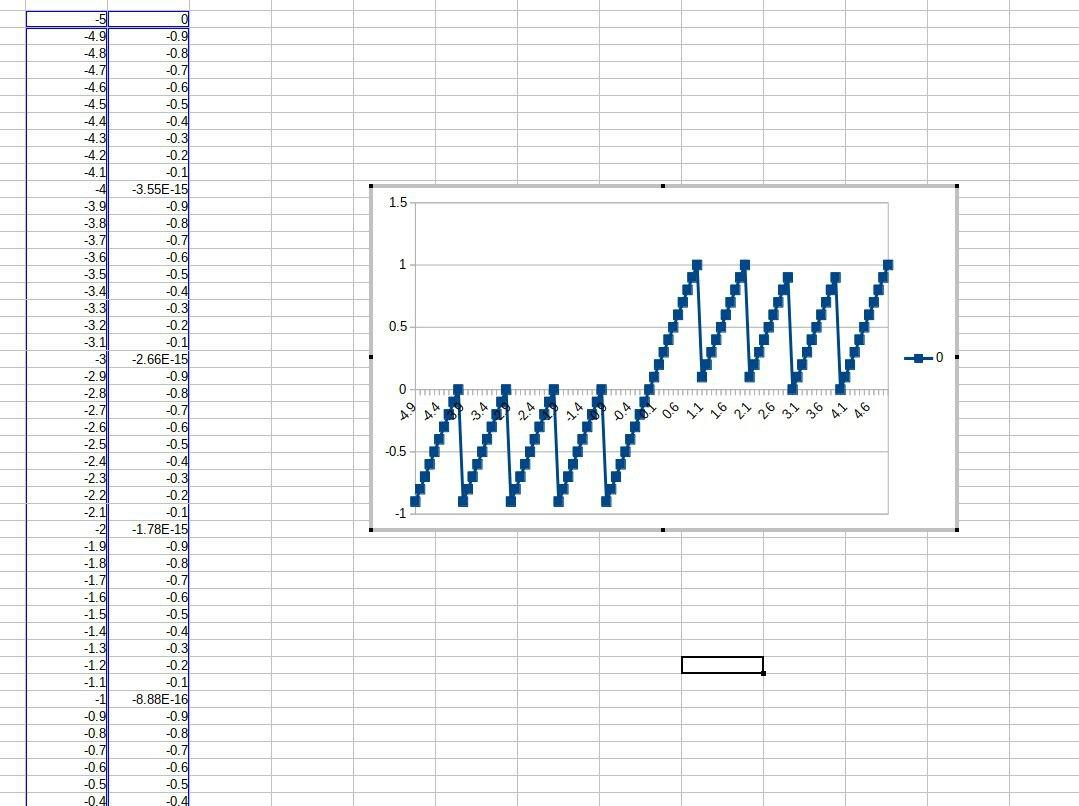
\includegraphics[scale=0.5]{excelplot}
  \caption{Plot fet amb un full de càlcul per comprovar el comportament de la funció fmod amb nombres negatius i positius. Al eix vertical es representa el resultat, i al horitzontal els valors d'entrada.}
\end{figure}

\section{Proves}
Degut a la naturalesa del projecte és prou complicat dissenyar tests unitaris. El correcte funcionament del motor s'ha comprovat a través del feedback visual de la demo.
Alguna de les funcionalitats testejables s'ha comprovat a través dels seus resultats, com és el cas de la simulació d'òrbites. L'escenari del joc conté una simulació del Sistema Solar a escala real, i per tant, de ser correcte la simulació les òrbites haurien de ser estables i similars a la realitat.
\\


En la figura \ref{mapaestelar} podem observar la representació de les òrbites de Mercuri, Venus, Terra, Mart i Júpiter, i s'observen les òrbites estables i amb cap tipus d'eccentricitat. Per la simulació s'han utilitzat les distàncies i velocitats mitjanes dels cossos, així que la eccentricitat real de les òrbites no queda reflectida en la simulació.
\begin{figure}[H]
  \centering
  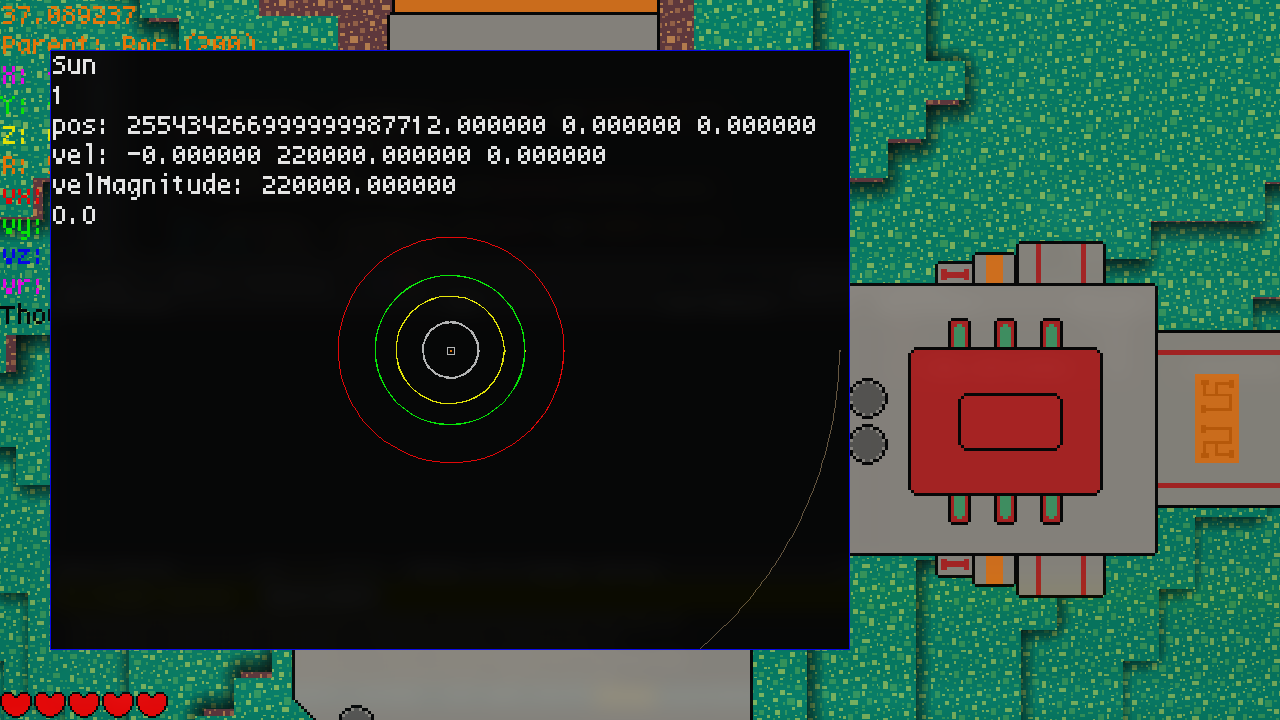
\includegraphics[scale=0.4]{orbites}
  \caption{Captura del mapa estelar.}
  \label{mapaestelar}
\end{figure}
%TODO com podem comprovar les òrbites dels principals planetes del sistema solar són estables i poc eccèntriques, amb el que podem establir que la simulació s'adiu prou correctament a la realitat.


